\documentclass[10pt,letterpaper]{article}

\usepackage{fontspec}
\setmainfont{texgyretermes-regular.otf}[BoldFont=texgyretermes-bold.otf,ItalicFont=texgyretermes-italic.otf,BoldItalicFont=texgyretermes-bolditalic.otf]
\usepackage{unicode-math}
\setmathfont{texgyretermes-math.otf}

\usepackage[letterpaper,margin=1in]{geometry}
\usepackage{amsmath}
\usepackage{graphicx}
\usepackage{booktabs}
\usepackage{array}
\usepackage{tabularx}
\usepackage[font=small,labelfont=bf,justification=raggedright,singlelinecheck=false]{caption}
\usepackage{microtype}
\usepackage[hidelinks]{hyperref}
\hypersetup{
  pdftitle={The Width Tax: Electrical, Package, and Thermal Limits of Bigger PCIe Links},
  pdfauthor={Amrendra Singh and DeepSeek V4.1 Flash 1017},
  pdfsubject={PCI Express, interconnect, SerDes, thermal, lane scaling},
  pdfkeywords={PCIe, lanes, SerDes, PAM4, interconnect, thermal}
}
\usepackage{titlesec}

\graphicspath{{../figures/}}

\setlength{\parindent}{1.2em}
\setlength{\parskip}{0pt}
\emergencystretch=1em

\titleformat{\section}{\large\bfseries}{\thesection.}{0.5em}{}
\titleformat{\subsection}{\normalsize\bfseries}{\thesubsection}{0.5em}{}
\titlespacing*{\section}{0pt}{1.5ex plus .3ex}{0.6ex}
\titlespacing*{\subsection}{0pt}{1.2ex plus .2ex}{0.3ex}

\begin{document}

\title{\textsc{\small Technical Report $\cdot$ Analysis Paper}\\[10pt]
\textbf{The Width Tax}\\[5pt]
{\large Electrical, Package, and Thermal Limits of Bigger PCIe Links}}
\author{\normalsize Amrendra Singh and DeepSeek V4.1 Flash 1017}
\date{\normalsize 2026}
\maketitle
\vspace{-1.4em}

\begin{abstract}
\noindent PCI Express scales bandwidth by adding lanes. The x16 connector has been the top of the CEM standard for two decades, and the obvious next step---x32---is blocked less by the protocol than by physics: pins, package escapes, crosstalk, SerDes power, and thermal density. This paper builds a first-order lane budget that treats width, rate, modulation, and reach as a single optimization. We show that each additional lane carries a superlinear width tax in connector density, package layers, and local thermal load; that the alternative---fewer, faster lanes---trades pins for channel loss and equalization power; that lane merging and width reduction are useful for yield, power, and latency-bound workloads but not for peak bandwidth; and that no lanes at all---optics, wireless, and package-level fabrics---wins at the extremes of reach. The result is a lane frontier: parallel buses at short reach, PCIe lanes in the middle, and optics beyond a few meters. The next PCIe generation should expose width, rate, and modulation as a tunable triad rather than treating lane count as the only scaling knob.
\end{abstract}

\noindent\textbf{Keywords:} PCI Express; lanes; SerDes; PAM4; interconnect; thermal; packaging.

\section{Introduction}
\label{sec:intro}

PCI Express has one scaling knob that system builders trust: add lanes. The x16 link has been the top of the CEM connector for two decades, and the bandwidth curve has been delivered by raising the per-lane rate, not by widening the link \cite{pcie6,pcie7,x16}. The next obvious step is x32. The protocol already permits it; the connector, the package, and the channel do not.

This paper argues that the lane is a middle-distance compromise. At short reach, a wide parallel bus is cheaper per bit; at long reach, optics is cheaper per meter; in between, PCIe's lane count is a reasonable but not optimal choice. Adding lanes at the top end buys bandwidth linearly and pays a superlinear width tax in pins, package escapes, crosstalk, power, and thermal density. The alternatives---fewer faster lanes, wider modulation, lane merging, and lane-less fabrics---each trade one tax for another.

Our contributions are five. First, we define a lane budget that treats width, rate, modulation, and reach as one optimization (Section~\ref{sec:budget}). Second, we quantify the width tax at x16, x32, and x64 (Section~\ref{sec:more}). Third, we analyze the three routes that avoid more lanes: fewer but faster lanes, wider modulation, and wider parallel lanes (Section~\ref{sec:fewer}). Fourth, we analyze lane merging and width reduction, including their effect on latency-bound memory traffic (Section~\ref{sec:merge}). Fifth, we analyze the lane-less alternatives---optics, wireless, package fabrics, and network fabrics---and combine everything into a lane frontier (Sections~\ref{sec:nolanes} and~\ref{sec:frontier}).

The method is analytical and first-order. We take rates, widths, and overheads from public specifications and published architecture descriptions, and we build a model rather than a calibrated simulator. The parameters are listed in the tables so that a reader can substitute their own. We do not report measurements, and we flag estimates as estimates.

\section{The Lane Budget}
\label{sec:budget}

\subsection{Definitions}

A lane is one differential pair carrying one serial stream. A link of width $N$ has $2N$ data wires plus sidebands and grounds. The lane rate $R$ is measured in gigabaud; the modulation $W$ is the number of bits per symbol (1 for NRZ, 2 for PAM4, 3 for PAM8); the efficiency $\eta$ accounts for encoding, framing, FEC, and protocol overhead. The link bandwidth is
\begin{equation}
B = N R W \eta.
\label{eq:bandwidth}
\end{equation}
Every route in this paper changes one of $N$, $R$, $W$, or $\eta$.

\subsection{Cost}

Cost is the sum of four terms:
\begin{equation}
P = N p(R,W) + p_{\mathrm{ret}}(L) + p_{\mathrm{conn}},
\label{eq:power}
\end{equation}
\begin{equation}
A = N a(R,W) + a_{\mathrm{conn}},
\label{eq:area}
\end{equation}
\begin{equation}
T = P R_{\mathrm{th}},
\label{eq:thermal}
\end{equation}
where $p$ is the per-lane SerDes power, $p_{\mathrm{ret}}$ the retimer power (zero below the reach limit), $a$ the per-lane package and connector area, and $R_{\mathrm{th}}$ the thermal resistance. The width tax is the derivative $\partial P/\partial N$: it is not constant, because crosstalk, equalization, and retimers grow with $N$.

\subsection{Reach}

Reach is set by the channel loss and the SNR budget:
\begin{equation}
L_{\max} = \frac{S - S_0}{\alpha(R,W)},
\label{eq:reach}
\end{equation}
where $S$ is the available SNR, $S_0$ the required SNR, and $\alpha$ the loss per meter. $\alpha$ grows with frequency and with the modulation order: PAM4 needs about 9.5~dB more SNR than NRZ at the same symbol rate, and PAM8 about 19~dB more \cite{pam4,shannon}.

\begin{table}[t]
\centering
\caption{PCIe generations. Bandwidth is one direction after encoding and framing; reach is a typical PCB limit without retimers and is an estimate.}
\label{tab:gens}
\small
\begin{tabularx}{\linewidth}{@{}lccccX@{}}
\toprule
Gen & Rate (GT/s) & Modulation & x16 (GB/s) & Per lane (GB/s) & Typical PCB reach \\
\midrule
1.0 & 2.5 & NRZ, 8b/10b & 4 & 0.25 & $\sim$1 m \\
2.0 & 5 & NRZ, 8b/10b & 8 & 0.50 & $\sim$0.5 m \\
3.0 & 8 & NRZ, 128b/130b & 15.75 & 0.98 & $\sim$0.3 m \\
4.0 & 16 & NRZ, 128b/130b & 31.5 & 1.97 & $\sim$0.2 m \\
5.0 & 32 & NRZ, 128b/130b & 63 & 3.94 & $\sim$0.15 m \\
6.0 & 64 & PAM4, FLIT/FEC & 121 & 7.56 & $\sim$0.1 m \\
7.0 & 128 & PAM4, FLIT/FEC & 242 & 15.1 & $\sim$0.05 m \\
\bottomrule
\end{tabularx}
\end{table}

\section{More Lanes: The Width Tax}
\label{sec:more}

\subsection{The connector}

The CEM connector has 164 pins. An x16 link uses 64 data pins (32 differential pairs), plus sidebands, grounds, and power. An x32 link needs 128 data pins; an x64 link needs 256. The connector is the first wall: a 328-pin or 656-pin edge connector is not a consumer part. Mating force, wipe, coplanarity, and cost all grow faster than the pin count. The connector is also where the channel is worst: the edge fingers, the vias, and the card-edge launch add reflections that the package and cable do not \cite{cem}.

\subsection{The package}

Each lane needs two bumps, a ground return, and an escape route. At a 0.8--1~mm bump pitch, 32 lanes consume 64 bumps plus grounds; 64 lanes consume 128. The escape routing consumes substrate layers, and the layers consume cost and yield. The package edge is the second wall: the die's beachfront is fixed, and the SerDes area grows with $N$.

\subsection{Electricity}

More lanes mean more aggressors. Near-end and far-end crosstalk grow with the number of adjacent pairs; ground pins must be interleaved; simultaneous switching noise grows with the number of drivers switching at once. The differential pair is not immune: the pair's own skew and the pair-to-pair coupling set the eye. At x32, the channel is a 64-pair bundle, and the bundle is a shared noise environment \cite{dally}.

\subsection{Power}

A 32~GT/s SerDes consumes roughly 50--100~mW per lane in 7~nm; 64~GT/s PAM4 roughly 100--150~mW. An x16 Gen6 link is 1.6--2.4~W; x32 is 3.2--4.8~W; x64 is 6.4--9.6~W. Add retimers at 1--2~W each: x32 needs two to four, x64 four to eight. The total is modest against a 75~W slot, but it is not free: at x64, 10~W is 13\% of the slot, and the card's compute budget shrinks.

\subsection{Thermal}

The thermal tax is local, not global. The connector and cable are often uncooled; their temperature rise is 10--20$^\circ$C, and the cable jacket is rated at 85$^\circ$C. The package hotspot is at the die edge, where the SerDes sits; the airflow shadow behind the connector is the worst place to put heat. At x64, the SerDes power is a small fraction of the card, but it is concentrated in the last centimeter, which is exactly where the thermal design is weakest \cite{ashrae}.

\subsection{Protocol}

More lanes mean more deskew, more L2/L3 state, more arbitration, and more training. The per-lane overhead is small, but the tag space does not scale with lanes: a single function still has 256 tags, and a cache-line fetch is still 64~bytes \cite{x16}. More lanes raise the link ceiling; they do not raise the latency bound.

\begin{figure}[t]
\centering
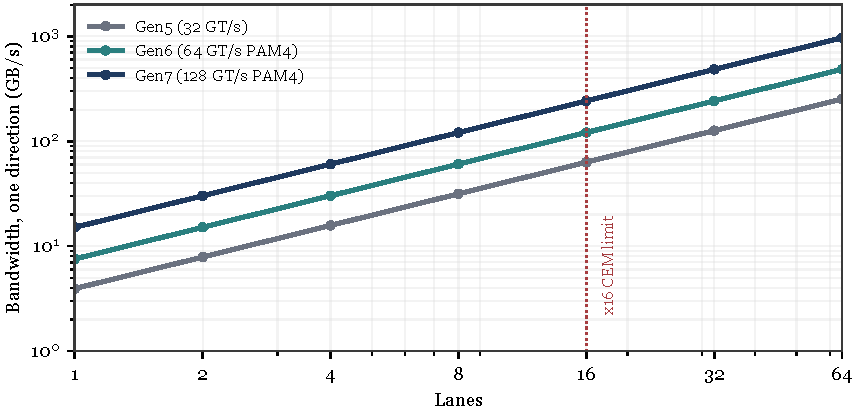
\includegraphics[width=\linewidth]{fig1_bandwidth.pdf}
\caption{Bandwidth versus lane count for Gen5, Gen6, and Gen7. The x16 point is the top of the CEM connector; x32 and x64 are protocol-permitted but connector-limited. The line is linear in $N$; the cost is not.}
\label{fig:bandwidth}
\end{figure}

\begin{figure}[t]
\centering
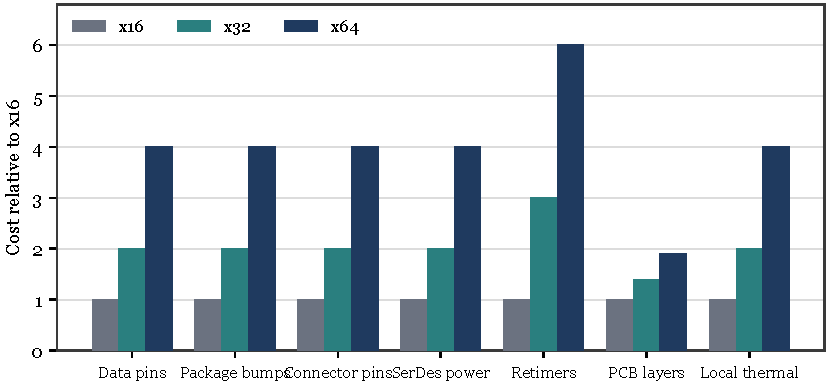
\includegraphics[width=\linewidth]{fig2_width_tax.pdf}
\caption{The width tax at x16, x32, and x64, normalized to x16. Pins and package bumps grow linearly; connector cost, retimer power, and local thermal density grow faster. The bars are first-order estimates.}
\label{fig:widthtax}
\end{figure}

\begin{table}[t]
\centering
\caption{The width tax at x16, x32, and x64. Values are first-order estimates for a Gen6-class SerDes; connector pin counts for x32 and x64 are hypothetical.}
\label{tab:width}
\small
\begin{tabularx}{\linewidth}{@{}lcccX@{}}
\toprule
Resource & x16 & x32 & x64 & Scaling \\
\midrule
Data pins & 64 & 128 & 256 & Linear \\
Ground pins & 32 & 64 & 128 & Linear \\
Package bumps & 64 & 128 & 256 & Linear \\
SerDes power (Gen6) & 1.6 W & 3.2 W & 6.4 W & Linear \\
Retimers & 0--2 & 2--4 & 4--8 & Superlinear \\
Connector pins & 164 & 328 & 656 & Linear, but impractical \\
PCB layers & 16 & 20--24 & 28--32 & Superlinear \\
Local thermal density & 1$\times$ & 2$\times$ & 4$\times$ & Linear in power, worse in airflow \\
\bottomrule
\end{tabularx}
\end{table}

\section{Fewer, Wider Lanes}
\label{sec:fewer}

\subsection{Wider modulation}

PAM4 doubles the bits per symbol at the same baud. It costs about 9.5~dB of SNR, which is why Gen6 pairs it with FEC and a flit-based framing \cite{pcie6}. PAM8 triples the bits per symbol and costs about 19~dB; at 32~GBd over a meter of FR4, the SNR is not there. The ``wider lane'' is really a deeper constellation, and it trades reach for rate.

\subsection{Higher rate}

Raising the baud from 32 to 64 to 128~GBd raises the loss. FR4 loses roughly 1~dB per inch at 16~GHz and 1.5~dB per inch at 32~GHz; the equalization budget is 20--30~dB, and beyond that the link needs a retimer or optics. The rate wall is the reach wall \cite{oif}.

\subsection{Fewer lanes at higher rate}

An x8 link at 64~GT/s PAM4 carries the same bandwidth as an x16 link at 32~GT/s NRZ. It halves the pins and the connector, but it doubles the per-lane rate, halves the reach, and raises the per-lane power. This is the ``less but wider'' route: fewer, faster lanes. It is the right choice when the connector is the bottleneck and the channel is short.

\subsection{Wider parallel lanes}

The other meaning of ``wider'' is more wires per lane at a lower rate: a 16-bit-wide lane at 8~GT/s carries 128~Gb/s over 32 wires and a clock. It has no SerDes, no CDR, no equalization; it is a source-synchronous bus. It is the right choice at package and board reach, and it is what HBM and UCIe do \cite{hbm,ucie}. The lane disappears into a bus.

\begin{figure}[t]
\centering
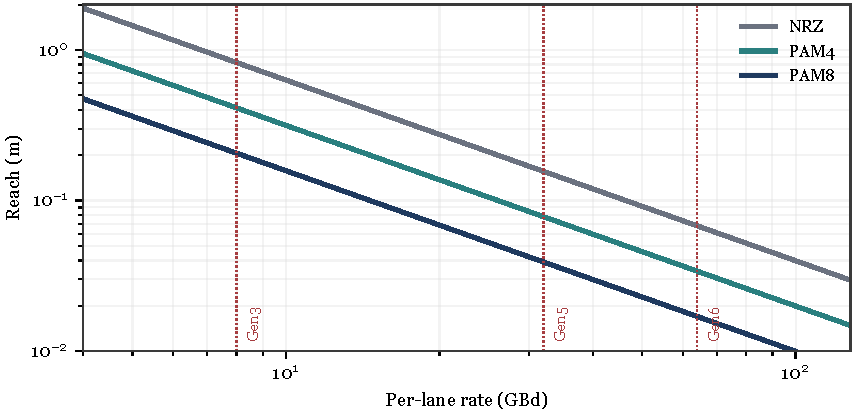
\includegraphics[width=\linewidth]{fig3_reach.pdf}
\caption{Reach versus per-lane rate for NRZ, PAM4, and PAM8. The curves are first-order loss budgets; the markers are PCIe generations. Higher modulation buys rate at the cost of reach, which is why Gen6 needs FEC and why Gen7 needs short channels.}
\label{fig:reach}
\end{figure}

\begin{table}[t]
\centering
\caption{Routes for scaling a link. Each changes a different variable in $B = N R W \eta$ and pays a different tax.}
\label{tab:routes}
\small
\begin{tabularx}{\linewidth}{@{}lccccX@{}}
\toprule
Route & Bandwidth & Pins & Power & Reach & Verdict \\
\midrule
More lanes & Linear & Linear & Linear & Same & Short reach only \\
Faster lanes & Linear & Same & Superlinear & Lower & Long reach with optics \\
PAM4 & 2$\times$ & Same & + & Lower & Gen6 default \\
PAM8 & 3$\times$ & Same & ++ & Much lower & Not yet \\
Wider parallel & Linear & Linear & Lower/bit & Short & Package and board \\
Merge 2:1 & Same & Half & Same/higher & Lower & Connector niche \\
Halve width & Half & Half & Half & Same & Power and thermal \\
No lanes & Depends & Zero & Depends & Extreme & Package and network \\
\bottomrule
\end{tabularx}
\end{table}

\section{Merging Lanes and Reducing Width}
\label{sec:merge}

\subsection{Aggregation}

Lane aggregation combines physical lanes into one logical link. Reducing width from x16 to x8 halves the bandwidth and halves the pins and power. The latency is unchanged; the tag space is unchanged; the concurrency is unchanged. For latency-bound traffic, the effective bandwidth is the minimum of the link ceiling and the latency bound \cite{x16}; reducing width does not hurt until the link ceiling falls below the latency bound.

\subsection{The effect}

Figure~\ref{fig:widtheffect} shows the effective bandwidth versus width for two workloads: 64-byte cache-line traffic with 256 tags at 1~$\mu$s, and 4~KB streaming traffic. The cache-line workload saturates at x4; the streaming workload scales with width. The lesson: width should be matched to the workload, not maximized.

\begin{figure}[t]
\centering
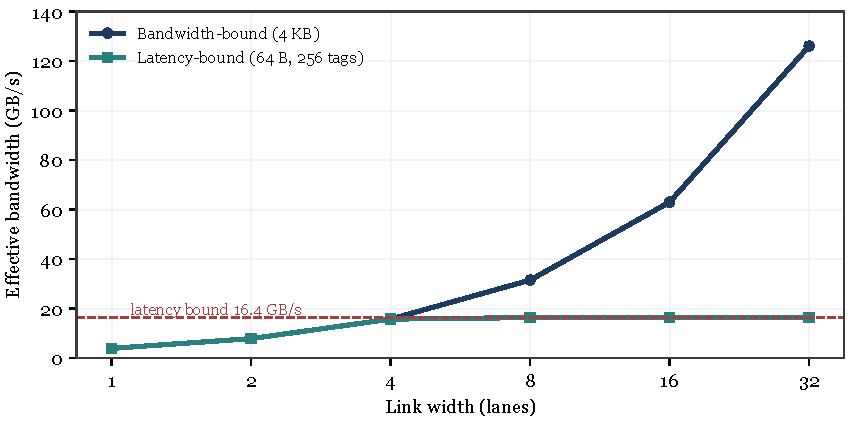
\includegraphics[width=\linewidth]{fig4_width_effect.pdf}
\caption{Effective bandwidth versus link width for a latency-bound cache-line workload and a bandwidth-bound streaming workload. Beyond x4, the cache-line workload gains nothing from more lanes; the streaming workload scales linearly.}
\label{fig:widtheffect}
\end{figure}

\subsection{Merging two lanes into one}

Combining two lanes into one at twice the rate keeps the bandwidth and halves the pins, but doubles the per-lane rate, halves the reach, and raises the per-lane power. It is a connector and package optimization, not a bandwidth optimization.

\subsection{Failover and dynamic width}

PCIe already negotiates width. A broken lane reduces the link to x8 or x4; the system degrades gracefully. Dynamic width can also trade bandwidth for power: idle lanes can be turned off, and the link can widen when the workload needs it. The cost is training time and protocol complexity \cite{pcie6}.

\subsection{Recommendation}

Match width to workload: x4--x8 for cache-line memory at microsecond latency, x16 for bandwidth-bound streaming, x32 only for short-reach backplanes where the connector is not the limit.

\section{No Lanes at All}
\label{sec:nolanes}

\subsection{Optics}

An optical link has no electrical lanes. It has wavelengths, fibers, and lanes in the WDM sense. The reach is 10~m to 10~km; the energy is 5--15~pJ/bit; the latency is set by the conversion, not the fiber. Co-packaged optics moves the conversion to the package, removing the electrical reach limit. The lane becomes a wavelength \cite{miller,cpo}.

\subsection{Wireless}

60~GHz wireless carries 1--10~Gb/s over 1--10~m with no lanes and no connector. It is a niche for rotation and reconfiguration, not for memory.

\subsection{Package-level}

UCIe, HBM, and NVLink use no PCIe lanes. They use bumps, interposers, and short traces: 0.5--5~mm, 1--2~Tb/s, sub-10~ns. The lane becomes a bump. This is the fastest growing part of the interconnect space, and it is where the width tax is paid in silicon area rather than pins \cite{ucie,hbm,nvlink}.

\subsection{Network fabrics}

CXL over Ethernet and RDMA use no dedicated lanes; they use a shared network. The reach is 100~m to 10~km; the latency is 10--100~$\mu$s; the bandwidth is 100--400~Gb/s per port. The lane becomes a packet \cite{cxl}.

\subsection{Power-line communication}

Data over the power delivery network uses no data lanes; it modulates the power pins. The bandwidth is Mbps, the reach is meters, and the noise is the VRM. It is a research route, not a memory route.

\begin{table}[t]
\centering
\caption{Lane-less alternatives. Reach, bandwidth, and latency are order-of-magnitude; the last column is the regime where each wins.}
\label{tab:laneless}
\small
\begin{tabularx}{\linewidth}{@{}lccccX@{}}
\toprule
Technology & Reach & Bandwidth & Latency & Maturity & Regime \\
\midrule
Optics & 10 m--10 km & 100 Gb/s--1.6 Tb/s & 100--500 ns & Mature & Long reach \\
Wireless 60 GHz & 1--10 m & 1--10 Gb/s & 100 ns & Niche & Rotation, reconfiguration \\
UCIe & 0.5--2 mm & 1--2 Tb/s & $<$10 ns & Emerging & Package \\
HBM & $\sim$5 mm & 1.2 TB/s & $<$10 ns & Mature & Interposer \\
CXL over Ethernet & 100 m--10 km & 100--400 Gb/s & 10--100 $\mu$s & Emerging & Shared network \\
Power-line data & 1--10 m & 1--100 Mb/s & 10 $\mu$s & Research & Power pins \\
\bottomrule
\end{tabularx}
\end{table}

\section{The Lane Frontier}
\label{sec:frontier}

\subsection{The design space}

The four variables are $N$, $R$, $W$, and $L$. The constraints are bandwidth $B_0$, reach $L_0$, power $P_0$, and pins $N_0$. The optimization is
\begin{equation}
\min_{N,R,W} P \quad \text{s.t.} \quad N R W \eta \ge B_0,\; L_{\max}(R,W) \ge L_0,\; N \le N_0.
\label{eq:opt}
\end{equation}

\subsection{The frontier}

The solution has a simple shape. At short reach, $N^*$ is large and $R^*$ is low: a parallel bus. At long reach, $N^*$ is small and $R^*$ is high: a serial lane with optics. In the middle, PCIe's lane count is a compromise. The width tax makes x32 and x64 unattractive except at the short-reach end.

\subsection{The regions}

Figure~\ref{fig:frontier} maps the frontier. The parallel-bus region is below 1~cm; the PCIe region is 0.1--3~m; the optics region is above 10~m; the wireless and network region is the no-lane extreme. The boundaries are not sharp, but the trend is.

\begin{figure}[t]
\centering
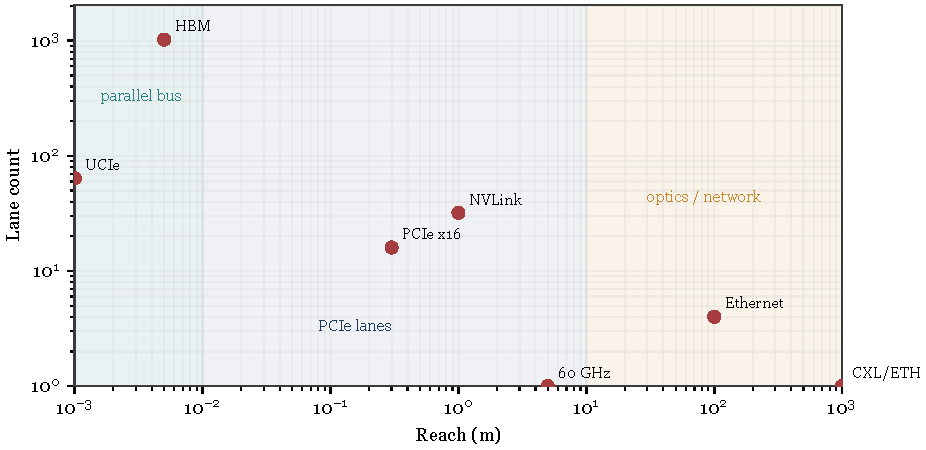
\includegraphics[width=\linewidth]{fig5_frontier.pdf}
\caption{The lane frontier: lane count versus reach, with the regions where parallel buses, PCIe lanes, optics, and lane-less fabrics win. The markers are representative technologies, not products.}
\label{fig:frontier}
\end{figure}

\subsection{The lesson}

The lane is not a law of nature; it is a packaging choice. The next PCIe generation should expose width, rate, and modulation as a triad, and it should let the platform choose the point on the frontier.

\section{Recommendations}
\label{sec:recs}

\begin{enumerate}
\item \textbf{Expose the triad.} Let a link negotiate width, rate, and modulation independently, so a platform can choose x8 at 64~GT/s, x4 at 128~GT/s, or x16 at 32~GT/s.
\item \textbf{Use modular connectors.} Two x8 connectors are cheaper and more flexible than one x16; four x8 connectors are the practical version of x32.
\item \textbf{Make width thermal-aware.} Turn off idle lanes; widen when the workload needs bandwidth; use width as a power knob.
\item \textbf{Use co-packaged optics for long reach.} Do not try to extend copper beyond the reach wall; move the conversion to the package.
\item \textbf{Standardize lane-less fabrics.} UCIe for the package, CXL over Ethernet for the network, and a clear boundary between them.
\item \textbf{Measure energy per bit per lane.} Bandwidth per pin is the wrong metric; energy per bit per meter is the right one.
\end{enumerate}

\section{Conclusion}
\label{sec:conclusion}

More lanes is the obvious answer, and it is the wrong one at both ends of the reach spectrum. At short reach, a wide parallel bus is cheaper; at long reach, optics is cheaper; in the middle, PCIe's lane count is a compromise that the width tax makes increasingly expensive. The next decade of interconnect will be won by matching width to reach, not by maximizing lane count. The lane is a means, not an end.

\begin{thebibliography}{99}

\bibitem{pcie6} PCI-SIG, \emph{PCI Express Base Specification, Revision 6.0}, 2022.

\bibitem{pcie7} PCI-SIG, \emph{PCI Express Base Specification, Revision 7.0}, 2025.

\bibitem{cem} PCI-SIG, \emph{PCI Express Card Electromechanical Specification, Revision 5.0}, 2022.

\bibitem{x16} A. Singh and DeepSeek V4.1 Flash, ``The x16 Ceiling: Connector, Silicon, and Latency Constraints on Memory Bandwidth over PCI Express,'' Technical Report, 2026.

\bibitem{cxl} CXL Consortium, \emph{Compute Express Link Specification, Revision 3.0}, 2022.

\bibitem{ucie} UCIe Consortium, \emph{Universal Chiplet Interconnect Express Specification, Revision 1.1}, 2023.

\bibitem{hbm} JEDEC, \emph{High Bandwidth Memory (HBM3E) Standard}, JESD238, 2023.

\bibitem{nvlink} NVIDIA, ``NVLink and NVSwitch,'' technical brief, 2024.

\bibitem{pam4} IEEE, \emph{IEEE 802.3bj}, 2014; and OIF, \emph{CEI-56G-PAM4}, 2017.

\bibitem{shannon} C. E. Shannon, ``A mathematical theory of communication,'' \emph{Bell System Technical Journal}, vol. 27, pp. 379--423, 1948.

\bibitem{dally} W. J. Dally and J. W. Poulton, \emph{Digital Systems Engineering}. Cambridge: Cambridge University Press, 1998.

\bibitem{oif} Optical Internetworking Forum, \emph{CEI-112G and CEI-224G Framework}, 2023.

\bibitem{ashrae} ASHRAE, \emph{Thermal Guidelines for Data Processing Environments}, 5th ed., 2021.

\bibitem{miller} D. A. B. Miller, ``Attojoule optoelectronics for low-energy information processing and communications,'' \emph{Journal of Lightwave Technology}, vol. 35, pp. 346--396, 2017.

\bibitem{cpo} M. H. Anderson \emph{et al.}, ``Co-packaged optics for data center switches,'' \emph{Journal of Lightwave Technology}, 2023.

\end{thebibliography}

\end{document}
